\section{Experiments}
\label{sec:experiments}

\subsection{Benchmark design}

The benchmark uses eight involutive conventions over two context bits
$(a_1, a_2)$: identity, NOT, and six XOR-with-context variants (full table
in Appendix~\ref{app:deferred-exp}). Each method receives a support set of
$K$ labelled (message, context, truth) triples per source and is evaluated
on held-out queries. All experiments use 10 seeds (0--9); we report mean
$\pm$ std. The statistics are exploratory: enough to separate stable gaps
from noise, not confirmatory tests.



\textbf{Baselines.} \emph{NoSupport} (content-only); \emph{UnsignedScalar}
(nonnegative weight, testing Theorem~\ref{thm:nonneg});
\emph{SignedScalar} (signed weight, testing Theorem~\ref{thm:scalar});
\emph{ContextConditioned} (Laplace context-matching);
\emph{CtxLogReg} (per-source context-dependent logistic weights);
\emph{MetaMean} and \emph{MetaAttn} (DeepSets-style neural calibrators);
\emph{Bayes} (the finite-grid aggregator of Section~\ref{sec:method}, with
\emph{BayesUniv}/\emph{BayesFam} variants in the K-sweep);
\emph{NaiveMean} and \emph{MajorityVote} (uncalibrated group rules); and the
\emph{Oracle} (true $(c_s,\rho_s,r_s)$, Bayes-optimal rule).

\subsection{Convention stability sweep}

We first vary the convention stability $\rho$ from $0.5$ (conventions
rarely applied) to $1.0$ (always applied), with $K=10$ and
$r \in [0.7, 0.95]$ (Table~\ref{tab:rhosweep}).

\begin{table}[h]
\centering
\footnotesize
\caption{Accuracy vs.\ convention stability $\rho$ ($K=10$); mean $\pm$ std over 10 seeds.}
\label{tab:rhosweep}
\resizebox{\columnwidth}{!}{
\begin{tabular}{rcccccc}
\toprule
$\rho$ & Bayes & MetaAttn & MetaMean & NoSupport & Signed & Unsigned \\
\midrule
0.5 & $0.625 \pm 0.011$ & $0.617 \pm 0.015$ & $0.621 \pm 0.012$ & $0.648 \pm 0.008$ & $0.616 \pm 0.012$ & $0.627 \pm 0.009$ \\
0.6 & $0.640 \pm 0.010$ & $0.629 \pm 0.014$ & $0.633 \pm 0.009$ & $0.624 \pm 0.010$ & $0.605 \pm 0.009$ & $0.610 \pm 0.006$ \\
0.7 & $0.659 \pm 0.010$ & $0.640 \pm 0.014$ & $0.645 \pm 0.010$ & $0.583 \pm 0.015$ & $0.591 \pm 0.011$ & $0.582 \pm 0.010$ \\
0.8 & $0.678 \pm 0.009$ & $0.648 \pm 0.014$ & $0.655 \pm 0.010$ & $0.545 \pm 0.010$ & $0.583 \pm 0.009$ & $0.560 \pm 0.009$ \\
0.9 & $0.714 \pm 0.011$ & $0.670 \pm 0.017$ & $0.682 \pm 0.012$ & $0.512 \pm 0.008$ & $0.603 \pm 0.011$ & $0.558 \pm 0.012$ \\
1.0 & $0.755 \pm 0.013$ & $0.696 \pm 0.028$ & $0.711 \pm 0.016$ & $0.482 \pm 0.023$ & $0.621 \pm 0.013$ & $0.554 \pm 0.015$ \\
\bottomrule
\end{tabular}
}
\end{table}

At low $\rho$ the conventions barely distort messages, so raw-message
methods hold their own (unsigned weighting reaches $0.627$ at
$\rho=0.5$). As $\rho \to 1$ the picture changes: NoSupport collapses
toward chance ($0.482$), unsigned and signed scalars stall, while the
Bayesian aggregator climbs monotonically to $0.755$ and the neural
calibrators partially recover ($0.696$--$0.711$). The price of ignoring
conventions grows with their stability, exactly as the theory predicts.
The per-query expected reliability ceiling under full convention
stability is $\mathbb{E}[r] = 0.825$ even for the oracle; the consensus
experiment (\S6.6) shows how independent sources combine to lift accuracy
far above that ceiling.

\begin{figure}[h]
\centering
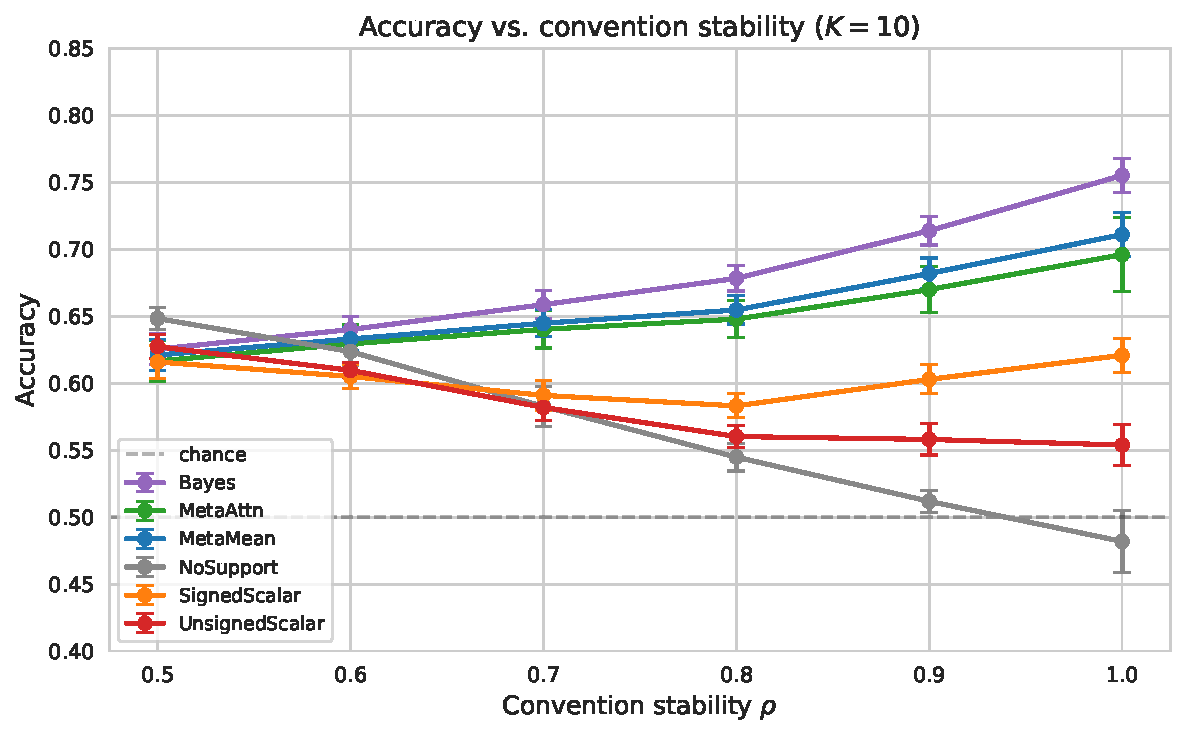
\includegraphics[width=0.8\columnwidth]{../figures/fig1_rho_sweep.pdf}
\caption{Accuracy vs.\ convention stability $\rho$ ($K=10$). Error bars show $\pm 1$ std over 10 seeds.}
\label{fig:rhosweep}
\end{figure}

\subsection{Representation ablation}

At $\rho \approx 1.0$ and $K=10$, accuracy follows the hierarchy predicted
by the theorems (Table~\ref{tab:ablation}, Figure~\ref{fig:ablation}):
content-only near chance, unsigned scalar low, signed scalar at $0.625$,
context-conditioned scalar at $0.730$, the attention calibrator at $0.722$,
the Bayesian aggregator at $0.758$, approaching the oracle at $0.825$.

\begin{table}[h]
\centering
\footnotesize
\caption{Representation ablation at $\rho \approx 1$, $K=10$; mean $\pm$ std over 10 seeds. Methods above the rule use only the support set available to every method; \textsc{Dec} and \textsc{DecCtx} below the rule receive ground-truth decoded features at inference and are diagnostics, not competitors.}
\label{tab:ablation}
\begin{tabular}{lc}
\toprule
Method & Accuracy \\
\midrule
\multicolumn{2}{c}{\textit{Deployable methods (support set only)}} \\
\midrule
ContentOnly & $0.537 \pm 0.033$ \\
UnsignedScalar & $0.550 \pm 0.006$ \\
SignedScalar & $0.625 \pm 0.014$ \\
ContextConditioned & $0.730 \pm 0.013$ \\
AttentionCalibrator & $0.722 \pm 0.013$ \\
Bayes & $0.758 \pm 0.015$ \\
EMDecoder (MAP point estimate) & $0.683 \pm 0.013$ \\
Oracle & $0.825 \pm 0.009$ \\
\midrule
\multicolumn{2}{c}{\textit{Privileged diagnostics (ground-truth decoded features)}} \\
\midrule
MetaAttn+Dec & $0.822 \pm 0.008$ \\
MetaAttn+DecCtx & $0.822 \pm 0.008$ \\
\bottomrule
\end{tabular}
\end{table}

{\sloppy
The table reads as a hierarchy that mirrors the theory: raw messages near
chance, unsigned scalars low (Theorem~\ref{thm:nonneg}), signed scalars at
$0.625$, context-conditioned scalars at $0.730$ (Theorem~\ref{thm:scalar}),
full latent-convention inference at $0.758$, and the oracle at $0.825$.
Two notes. First, our initial \textsc{ContextConditioned} baseline
silently collapsed to \textsc{SignedScalar}; we reimplemented it with
Laplace-smoothed context-matching support agreement. Second, the
diagnostic \textsc{MetaAttn+Dec} variants receive the true-convention-decoded
bit at inference and reach the oracle ceiling ($0.822$ vs.\ $0.825$), so
the learned calibrator's remaining gap is representational, not a
capacity problem. Finally, the hand-crafted
\textsc{ContextConditioned} ($0.730 \pm 0.013$) has overlapping 95\% CIs
with the higher-capacity \textsc{MetaAttn} ($0.722 \pm 0.013$), so the
observed difference is not clearly separated at this sample size.

A natural objection is that these baselines are too weak: a sufficiently
expressive source${}\times{}$context meta-learner might match Bayes
without generative machinery. \textsc{CtxLogReg} tests this: per-source
logistic regression on the same $K=10$ support set, with the logit a
context-dependent weight on the message,
$w_0 + m\,(v_0 + v_1a_1 + v_2a_2 + v_{12}a_1a_2)$, which nests
\textsc{ContextConditioned}'s per-context sign and can express any of the
eight conventions' decoding maps. It reaches only $0.637 \pm 0.007$,
below \textsc{ContextConditioned} and Bayes with non-overlapping CIs.
The result is not a regularisation artefact ($\lambda = 0.01$ and $0.1$
agree; accuracy rises with $K$, $0.63 \to 0.71$ from $K=10$ to $50$). At
$K=10$, expressiveness without the right inductive bias does not help.

A further ablation isolates \emph{why} Bayes beats the scalar baselines,
and answers the paper's central empirical question: does posterior
uncertainty matter beyond point-estimate decoding?
\textsc{EMDecoder} fits the same generative model by EM but decides with
the MAP convention and a plug-in log-odds weight: $0.683 \pm 0.013$,
\emph{below} \textsc{ContextConditioned}. Plugging the EM point estimates
into the exact oracle log-odds formula recovers $0.732 \pm 0.010$,
matching \textsc{ContextConditioned} but still $2.6$ points short of the
posterior-predictive $0.758$ (non-overlapping 95\% CIs). The generative
structure alone does not explain Bayes's performance: averaging over
convention uncertainty does independent work, and committing to a single
estimated convention (MAP recovery only $\approx 0.39$ at $K=10$) throws
away a further $4.9$ points. Explicit context conditioning recovers much
of the lost performance, but Bayesian inference over the latent
generative convention provides an additional advantage from uncertainty
marginalisation.
\par}

\begin{figure}[h]
\centering
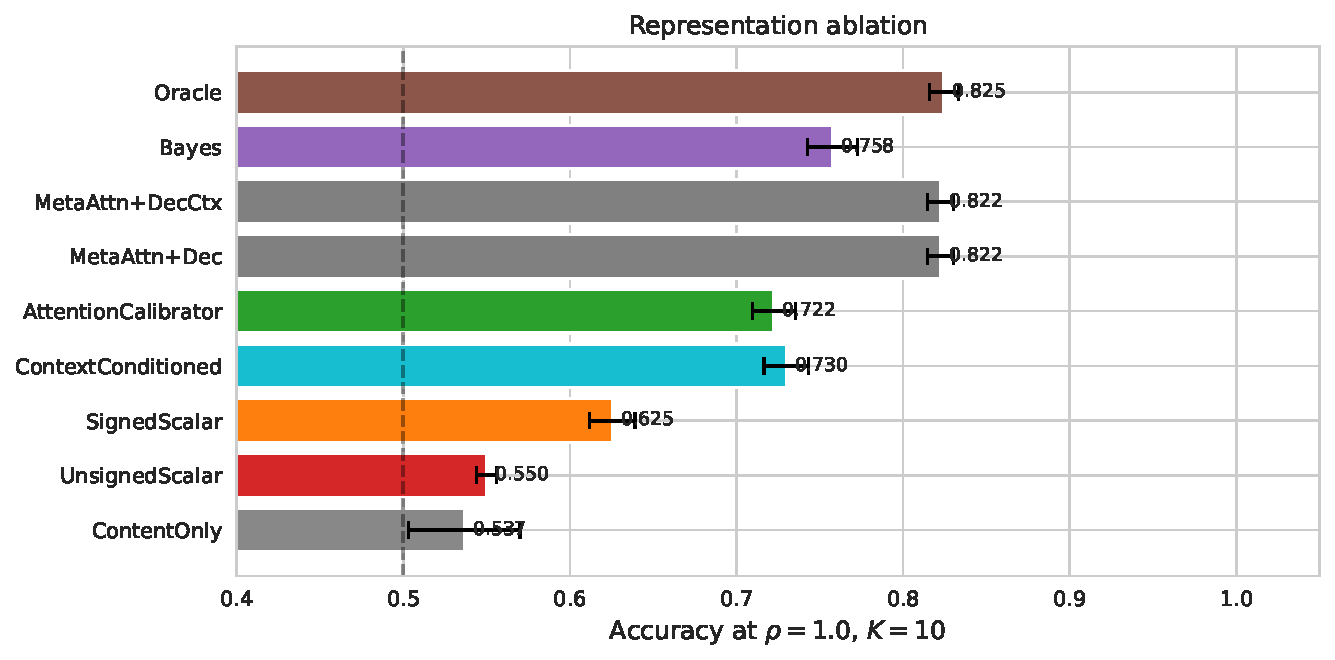
\includegraphics[width=0.8\columnwidth]{../figures/fig2_ablation.pdf}
\caption{Representation ablation at $\rho \approx 1$, $K=10$. Error bars show $\pm 1$ std over 10 seeds. Unsigned scalars fail (Theorem~\ref{thm:nonneg}); signed scalars fix inversion but not context-dependence (Theorem~\ref{thm:scalar}).}
\label{fig:ablation}
\end{figure}

\subsection{Support-size scaling on held-out conventions}

Test conventions $\{4, 5, 6, 7\}$; $K \in \{1, 2, 5, 10, 20, 50\}$
(support sets are nonempty, as the neural encoders require).
``Held-out'' means the following. The neural calibrators are trained on
sources using conventions $\{0, 1, 2, 3\}$ and evaluated on sources using
conventions $\{4, 5, 6, 7\}$, with $K$ labelled support examples per
source available at test time for calibration. \textsc{BayesUniv}
considers all eight conventions as candidates.
\textsc{BayesFam} restricts its candidate set to $\{4, 5, 6, 7\}$: it
knows the test family, and the comparison between the two Bayesian
variants therefore measures the value of that knowledge rather than
generalisation to unseen conventions.

\begin{table}[h]
\centering
\footnotesize
\caption{Accuracy on held-out conventions vs.\ support size $K$; mean $\pm$ std over 10 seeds.}
\label{tab:ksweep}
\resizebox{\columnwidth}{!}{
\begin{tabular}{rccccc}
\toprule
$K$ & BayesUniv & BayesFam & MetaAttn & MetaMean & NoSupport \\
\midrule
1  & $0.588 \pm 0.014$ & $0.647 \pm 0.019$ & $0.543 \pm 0.016$ & $0.523 \pm 0.019$ & $0.475 \pm 0.032$ \\
2  & $0.644 \pm 0.009$ & $0.687 \pm 0.015$ & $0.563 \pm 0.017$ & $0.559 \pm 0.013$ & $0.480 \pm 0.035$ \\
5  & $0.711 \pm 0.014$ & $0.741 \pm 0.014$ & $0.598 \pm 0.015$ & $0.578 \pm 0.012$ & $0.480 \pm 0.039$ \\
10 & $0.767 \pm 0.009$ & $0.786 \pm 0.010$ & $0.616 \pm 0.024$ & $0.589 \pm 0.009$ & $0.483 \pm 0.034$ \\
20 & $0.793 \pm 0.011$ & $0.805 \pm 0.010$ & $0.635 \pm 0.032$ & $0.603 \pm 0.014$ & $0.490 \pm 0.032$ \\
50 & $0.820 \pm 0.006$ & $0.822 \pm 0.006$ & $0.641 \pm 0.028$ & $0.621 \pm 0.016$ & $0.484 \pm 0.029$ \\
\bottomrule
\end{tabular}
}
\end{table}

Both Bayesian variants rise monotonically with $K$, converging to
approximately $0.82$ at $K=50$, which is, up to noise, the information
ceiling $\mathbb{E}[r] = 0.825$. The neural calibrators climb from chance
to $0.62$--$0.64$ and then flatline, a gap of roughly 18 percentage points
at $K=50$ under the tested conditions. We do not claim this bounds learned
calibrators in general; with matched support information and modest
capacity, structure beats learning here.



\begin{center}
\emph{[Figure omitted for space; see Appendix~\ref{app:deferred-exp}.]}
\end{center}


\subsection{Reliability heterogeneity}

$\rho \in [0.99, 1.0]$. The three regimes are
\emph{mean-matched}: homogeneous $r \in [0.79, 0.81]$, moderate $r \in
[0.70, 0.90]$, heterogeneous $r \in [0.65, 0.95]$, all with
$\mathbb{E}[r] = 0.80$. This matching matters: an earlier version of this
experiment let the heterogeneous regime have lower mean reliability as
well, so its performance drop could have been blamed on the level rather
than the spread. With the means matched, any remaining difference across
regimes is attributable to the \emph{spread} of reliabilities alone.

\begin{table}[h]
\centering
\footnotesize
\caption{Bayesian robustness to reliability heterogeneity (mean-matched, $\mathbb{E}[r]=0.80$); mean $\pm$ std over 10 seeds.}
\label{tab:rel}
\begin{tabular}{lccc}
\toprule
Regime & Bayes & MetaAttn & NoSupport \\
\midrule
Homogeneous   & $\mathbf{0.728 \pm 0.013}$ & $0.699 \pm 0.012$ & $0.596 \pm 0.009$ \\
Moderate      & $\mathbf{0.727 \pm 0.017}$ & $0.707 \pm 0.011$ & $0.589 \pm 0.010$ \\
Heterogeneous & $\mathbf{0.731 \pm 0.011}$ & $0.706 \pm 0.009$ & $0.593 \pm 0.006$ \\
\bottomrule
\end{tabular}
\end{table}

Bayes outperforms the baselines evaluated in this experiment across all
regimes, and its accuracy is flat at $\approx 0.73$ across spreads (all
three 95\% confidence intervals overlap). An ablation pinning reliability
to its mean ($r = 0.80$, convention and stability still inferred)
reproduces this flat profile exactly ($\Delta \leq 0.002$ in every
regime), so the flatness should not be attributed to per-source
reliability inference: it reflects robustness of convention
identification to reliability misspecification. (The per-query ceiling is
$\mathbb{E}[r] = 0.80$; the remaining gap is the usual cost of inferring
parameters from $K = 10$.)



\begin{center}
\emph{[Figure omitted for space; see Appendix~\ref{app:deferred-exp}.]}
\end{center}


\subsection{Multi-agent consensus}

$N$ agents observe a shared binary truth, each with its own $(c, \rho, r)$
sampled i.i.d.\ as follows:
$c_s \sim \mathrm{Uniform}(\mathcal{C})$,
$\rho_s \sim \mathrm{Uniform}([0.7, 1.0])$,
$r_s \sim \mathrm{Uniform}([0.7, 0.95])$.
The sampling distribution does not depend on $N$; realized diversity
increases with $N$ because more i.i.d.\ draws are combined.

\begin{table}[h]
\centering
\footnotesize
\caption{Group accuracy vs.\ number of agents under mixed conventions; mean $\pm$ std over 10 seeds.}
\label{tab:consensus}
\resizebox{\columnwidth}{!}{
\begin{tabular}{rcccc}
\toprule
$N$ & Naive & MetaAttn & Bayes & Oracle \\
\midrule
2  & $0.522 \pm 0.064$ & $0.742 \pm 0.061$ & $0.760 \pm 0.038$ & $0.825 \pm 0.062$ \\
3  & $0.528 \pm 0.049$ & $0.805 \pm 0.066$ & $0.798 \pm 0.056$ & $0.888 \pm 0.043$ \\
4  & $0.562 \pm 0.038$ & $0.832 \pm 0.059$ & $0.862 \pm 0.050$ & $0.910 \pm 0.042$ \\
6  & $0.575 \pm 0.062$ & $0.852 \pm 0.059$ & $0.883 \pm 0.047$ & $0.953 \pm 0.017$ \\
8  & $0.590 \pm 0.048$ & $0.903 \pm 0.027$ & $\mathbf{0.932 \pm 0.031}$ & $0.968 \pm 0.028$ \\
12 & $0.573 \pm 0.061$ & $0.937 \pm 0.033$ & $\mathbf{0.955 \pm 0.019}$ & $0.995 \pm 0.008$ \\
\bottomrule
\end{tabular}
}
\end{table}

Naive averaging sits near chance at every $N$: its sign \emph{is} the
majority vote, so the two coincide and we report a single column.
Both calibrated methods rise sharply with $N$; at $N=12$,
Bayes is within $4.0$ points of the oracle and $38.2$ points above
naive averaging. Bayes and MetaAttn have overlapping confidence intervals
at small $N$ ($0.805$ vs.\ $0.798$ at $N=3$, std $\approx 0.06$), so the
observed difference is not clearly separated at this sample size;
their point estimates separate from $N=8$ in Bayes's favour, though the gap
remains within noise through $N=12$. As $N$ grows the naive-to-calibrated
gap widens: more agents help only if you can decode them.

\begin{figure}[h]
\centering
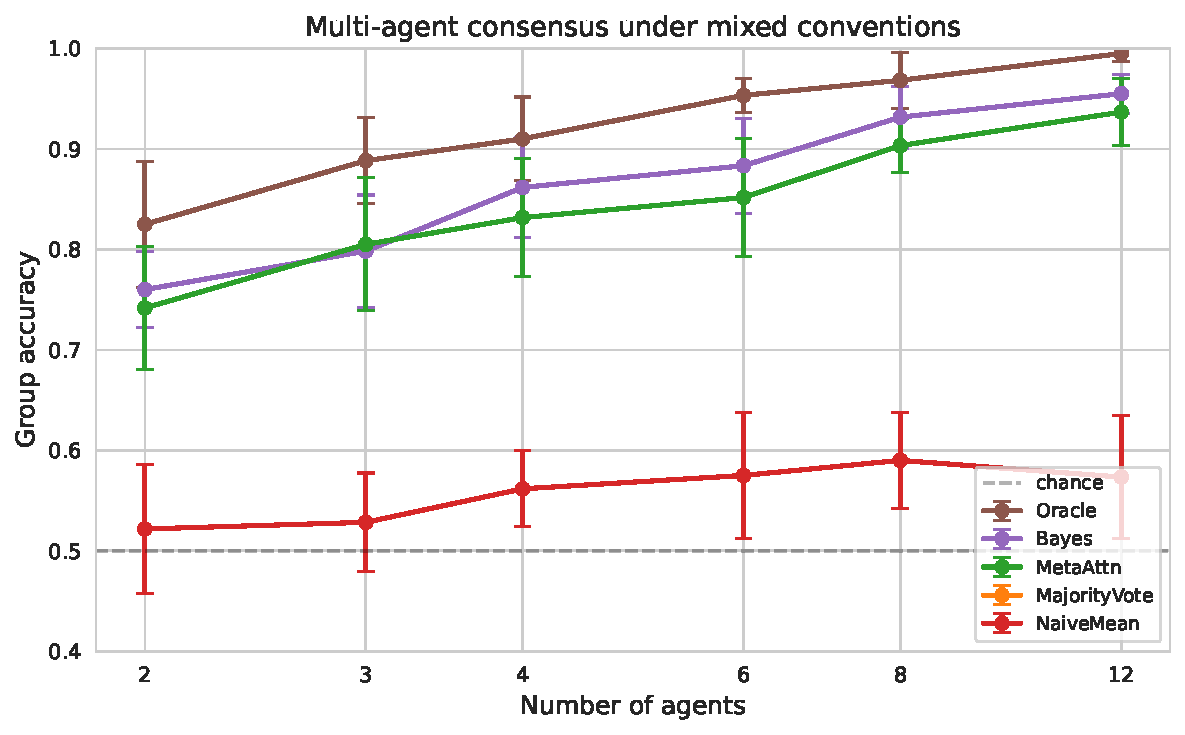
\includegraphics[width=0.8\columnwidth]{../figures/fig5_consensus.pdf}
\caption{Multi-agent consensus accuracy vs.\ number of agents. Error bars show $\pm 1$ std over 10 seeds.}
\label{fig:consensus}
\end{figure}

\subsection{Candidate-set misspecification}

In practice the modeller never knows the full convention family, so we
stress-test a wrong candidate set: sources drawn from all eight
conventions while the Bayesian candidate set is restricted to
$\{0, 1, 2, 3\}$ (\emph{BayesHalf}); \emph{BayesFull} (all eight) is the
well-specified control. $\rho \in [0.99, 1.0]$, $r \in [0.7, 0.95]$,
$K = 10$. We report overall accuracy plus the split by whether the true
convention was inside the candidate set.

\begin{table}[h]
\centering
\footnotesize
\caption{Accuracy under candidate-set misspecification; mean $\pm$ std over 10 seeds. \emph{BayesHalf} splits accuracy by whether the true convention was inside its candidate set.}
\label{tab:misspec}
\begin{tabular}{lc}
\toprule
Method & Accuracy \\
\midrule
BayesFull & $0.756 \pm 0.013$ \\
BayesHalf & $0.685 \pm 0.012$ \\
\quad in-candidate ($c \in \{0..3\}$) & $0.767 \pm 0.015$ \\
\quad out-of-candidate ($c \in \{4..7\}$) & $0.599 \pm 0.020$ \\
MetaAttn & $0.731 \pm 0.010$ \\
Oracle & $0.824 \pm 0.007$ \\
\bottomrule
\end{tabular}
\end{table}

\begin{figure}[h]
\centering
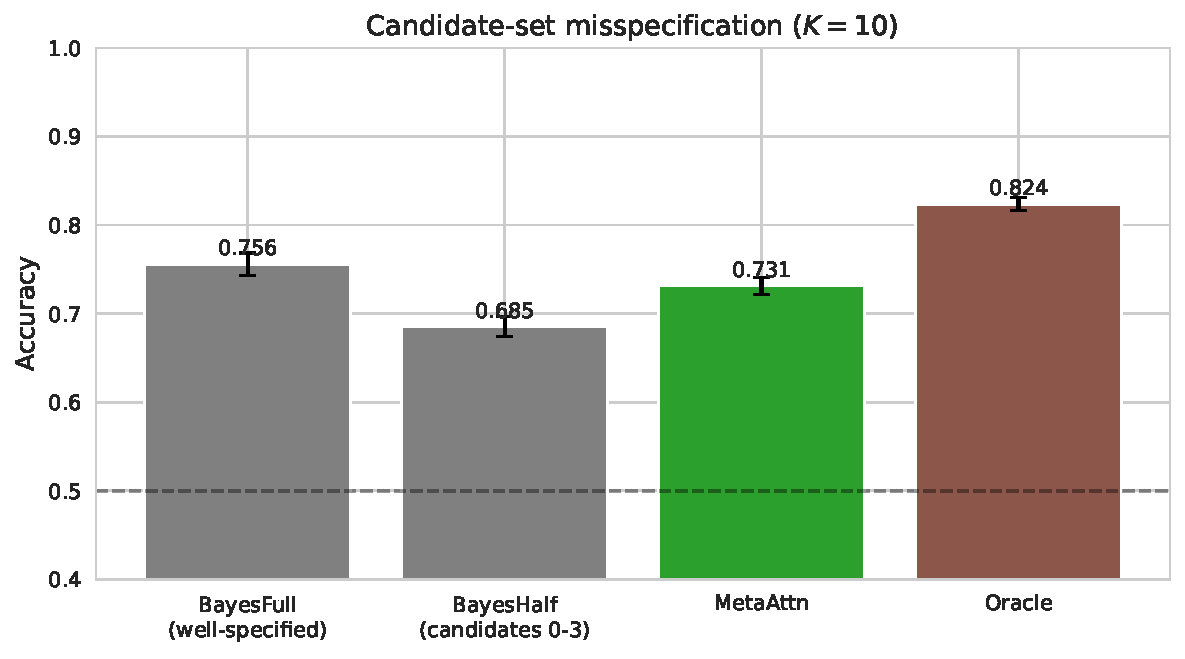
\includegraphics[width=0.8\columnwidth]{../figures/fig6_misspec.pdf}
\caption{Accuracy under candidate-set misspecification ($K=10$). Error bars show $\pm 1$ std over 10 seeds.}
\label{fig:misspec}
\end{figure}

Performance decreases from $0.756$ to $0.685$ overall, with the reduction
concentrated on sources whose true convention lies outside the candidate
set. On in-candidate sources the restricted model matches the
well-specified control ($0.767$ vs.\ $0.756$, within noise); on
out-of-candidate sources accuracy falls to $0.599$, still well above
chance, since the posterior spreads mass over the nearest available
conventions rather than committing to a single wrong one. Overall
\textsc{BayesHalf} drops $7$ points ($0.685$ vs.\ $0.756$).
Notably, the learned \textsc{MetaAttn} ($0.731$) lands between the two
Bayesian variants: with no convention family assumed, it handles
misspecification better than the restricted Bayesian but worse than the
well-specified one. The Bayesian aggregator is a closed-world method,
strong inside its assumed family; this experiment bounds the cost of
getting the family wrong.

\subsection{Correlated sources: breaking the independence assumption}

Every result so far keeps the model correctly specified. Here it is
deliberately \emph{not} the data-generating process: the Bayesian
aggregator assumes sources are conditionally independent given the truth,
so we correlate their errors. Ten sources (five pairs) report on one
shared truth per query; within-pair query-time errors correlate at
$\approx 0.5$ (Gaussian copula, calibrated; measured $0.44$--$0.52$),
with ExpB draws otherwise ($\rho \in [0.99, 1.0]$, $r \in [0.7, 0.95]$,
$K = 10$). Support data stay independent, isolating the misspecification
to the combination step. A paired-seed independence arm is the control;
\textsc{MetaAttn} could not be re-run here (torch unavailable). Correlation
costs every method about a point, \emph{including the oracle}, which also
sums independent log-odds: Bayes $0.971 \to 0.958$,
\textsc{ContextConditioned} $0.962 \to 0.950$,
\textsc{SignedScalar} $0.847 \to 0.844$, naive $0.449 \to 0.457$, Oracle
$0.994 \to 0.983$ (mean $\pm$ 95\% CI over 10 seeds; paired per-seed deltas
$-0.013$, $-0.012$, $-0.004$, $+0.008$, $-0.011$, all within noise of each
other). The problem itself gets harder under correlation, and Bayes is
not disproportionately hurt: the ranking Bayes ${} > {}$
\textsc{ContextConditioned} ${} > {}$ \textsc{SignedScalar} ${} > {}$
naive is preserved in both arms.
